% --------------------------------------------------------------------------- %
% Poster for the ECCS 2011 Conference about Elementary Dynamic Networks.      %
% --------------------------------------------------------------------------- %
% Created with Brian Amberg's LaTeX Poster Template. Please refer for the     %
% attached README.md file for the details how to compile with `pdflatex`.     %
% --------------------------------------------------------------------------- %
% $LastChangedDate:: 2011-09-11 10:57:12 +0200 (V, 11 szept. 2011)          $ %
% $LastChangedRevision:: 128                                                $ %
% $LastChangedBy:: rlegendi                                                 $ %
% $Id:: poster.tex 128 2011-09-11 08:57:12Z rlegendi                        $ %
% --------------------------------------------------------------------------- %
\documentclass[a0paper,landscape]{baposter}

\usepackage{relsize}		% For \smaller
\usepackage{url}			% For \url
\usepackage{epstopdf}	% Included EPS files automatically converted to PDF to include with pdflatex
\usepackage{natbib}

%%% Global Settings %%%%%%%%%%%%%%%%%%%%%%%%%%%%%%%%%%%%%%%%%%%%%%%%%%%%%%%%%%%

\graphicspath{{./}}	% Root directory of the pictures 
\tracingstats=2			% Enabled LaTeX logging with conditionals

%%% Color Definitions %%%%%%%%%%%%%%%%%%%%%%%%%%%%%%%%%%%%%%%%%%%%%%%%%%%%%%%%%

\definecolor{bordercol}{RGB}{40,40,40}
\definecolor{headercol1}{RGB}{186,215,230}
\definecolor{headercol2}{RGB}{0,60,255}
\definecolor{headerfontcol}{RGB}{0,0,0}
\definecolor{boxcolor}{RGB}{186,215,230}

%%%%%%%%%%%%%%%%%%%%%%%%%%%%%%%%%%%%%%%%%%%%%%%%%%%%%%%%%%%%%%%%%%%%%%%%%%%%%%%%
%%% Utility functions %%%%%%%%%%%%%%%%%%%%%%%%%%%%%%%%%%%%%%%%%%%%%%%%%%%%%%%%%%

%%% Save space in lists. Use this after the opening of the list %%%%%%%%%%%%%%%%
\newcommand{\compresslist}{
	\setlength{\itemsep}{1pt}
	\setlength{\parskip}{0pt}
	\setlength{\parsep}{0pt}
}

%%%%%%%%%%%%%%%%%%%%%%%%%%%%%%%%%%%%%%%%%%%%%%%%%%%%%%%%%%%%%%%%%%%%%%%%%%%%%%%
%%% Document Start %%%%%%%%%%%%%%%%%%%%%%%%%%%%%%%%%%%%%%%%%%%%%%%%%%%%%%%%%%%%
%%%%%%%%%%%%%%%%%%%%%%%%%%%%%%%%%%%%%%%%%%%%%%%%%%%%%%%%%%%%%%%%%%%%%%%%%%%%%%%

\begin{document}
\typeout{Poster rendering started}

%%% Setting Background Image %%%%%%%%%%%%%%%%%%%%%%%%%%%%%%%%%%%%%%%%%%%%%%%%%%
\background{
	\begin{tikzpicture}[remember picture,overlay]%
	\draw (current page.north west)+(-2em,2em) node[anchor=north west]
	{\includegraphics[height=1.1\textheight]{background}};
	\end{tikzpicture}
}

%%% General Poster Settings %%%%%%%%%%%%%%%%%%%%%%%%%%%%%%%%%%%%%%%%%%%%%%%%%%%
%%%%%% Eye Catcher, Title, Authors and University Images %%%%%%%%%%%%%%%%%%%%%%
\begin{poster}{
	grid=false,
	% Option is left on true though the eyecatcher is not used. The reason is
	% that we have a bit nicer looking title and author formatting in the headercol
	% this way
	eyecatcher=true, 
	borderColor=bordercol,
	headerColorOne=headercol1,
	headerColorTwo=headercol2,
	headerFontColor=headerfontcol,
	% Only simple background color used, no shading, so boxColorTwo isn't necessary
	boxColorOne=boxcolor,
	headershape=roundedright,
	headerfont=\Large\sf\bf,
	textborder=rectangle,
	background=user,
	headerborder=open,
  boxshade=plain
}
%%% Eye Cacther %%%%%%%%%%%%%%%%%%%%%%%%%%%%%%%%%%%%%%%%%%%%%%%%%%%%%%%%%%%%%%%
{
\includegraphics[width=6em,height=6em]{jayhawk}
}
%%% Title %%%%%%%%%%%%%%%%%%%%%%%%%%%%%%%%%%%%%%%%%%%%%%%%%%%%%%%%%%%%%%%%%%%%%
{\bf
	Algorithms for Calculating Pattern Class Probabilities on Phylogenetic Trees
}
%%% Authors %%%%%%%%%%%%%%%%%%%%%%%%%%%%%%%%%%%%%%%%%%%%%%%%%%%%%%%%%%%%%%%%%%%
{
	\vspace{1em} Jordan M. Koch and Mark T. Holder\\
	{\smaller \url{j772k779@ku.edu}, \url{mtholder@ku.edu}}
}
%%% Logo %%%%%%%%%%%%%%%%%%%%%%%%%%%%%%%%%%%%%%%%%%%%%%%%%%%%%%%%%%%%%%%%%%%%%%
{
% The logos are compressed a bit into a simple box to make them smaller on the result
% (Wasn't able to find any bigger of them.)

\setlength\fboxsep{0pt}
\setlength\fboxrule{0.5pt}
	\fbox{
		\begin{minipage}{6em}
			%\includegraphics[width=10em,height=4em]{colbud_logo}
			%\includegraphics[width=4em,height=4em]{elte_logo} \\
			%\includegraphics[width=10em,height=4em]{dynanets_logo}
			\includegraphics[width=6em,height=6em]{imsdlogo}
		\end{minipage}
	}
}

\headerbox{Introduction}{name=intro,column=0,row=0}{
A wide variety of evolutionary analyses are based upon the coupling of phylogenetic trees with models of how biological traits change during evolution. 
Felsenstein's \citep{Felsenstein1981} pruning algorithm makes it feasible to calculate the probability of any particular pattern of data arising on a phylogeny. 
In some contexts, one needs to calculate the probability that any member of a broad class of patterns will arise on the tree. 
For example, the model adequacy approach of Waddell et al. (2009) requires calculating the probability of several classes of patterns.  
Extending the morphological models of Lewis \citep{Lewis2001} to deal with many data sets requires calculating the probability of any parsimony-informative pattern arising (`parsimony' referring to the simplest explanation of the data, and parsimony-informative referring to those patterns which affect phylogenetic estimation). Application of the approaches of Waddell {\em et al.~}\citep{WaddellOP2009} and Lewis\citep{Lewis2001} are limited because the only known methods for calculating the probability of a class of patterns involve either simulating a large amount of data or exhaustively considering every member of the class. Neither approach is feasible on large trees.

We are developing dynamic programming algorithms to calculate the probabilities of pattern classes in one pass down a phylogenetic tree. The algorithms include a general approach (applicable to any standard model of character evolution) as well as optimizations for the fully symmetric models (e.g. those of Lewis\citep{Lewis2001}). We are implementing these algorithms in open source software written in C++, and plan to include the approaches in the GARLI \citep{GARLI} software package for use in inferring evolutionary trees.
%
}

\headerbox{Research Goals}{name=research goals,column=0,below=intro}{
\begin{itemize}
\item We are working to discover algorithms which will calculate the probabilities of classes of patterns in phylogenetic binary trees.  
\item In particular, we are striving to implement these algorithms towards the specialization for symmetric models.  This will involve identifiying several tricks.  Recognizing these symmetric cases will simplify the code, causing it to run more efficiently and accurately in the C++ open source software.
\end{itemize}
}

\headerbox{Results for the General Algorithm}{name=results,span=2,column=1,row=0}{
Waddell {\em et al.~}\citep{WaddellOP2009} used simulation in his tables to obtain expected probability values.  We tested our algorithm with the same data and obtained very similar values.  This figure represents a phylogenetic tree which uses this data to perform pairwise tests.  In this figure, long branches simplify many changes; the character states in these branches' DNA are much different than in other branches.\\
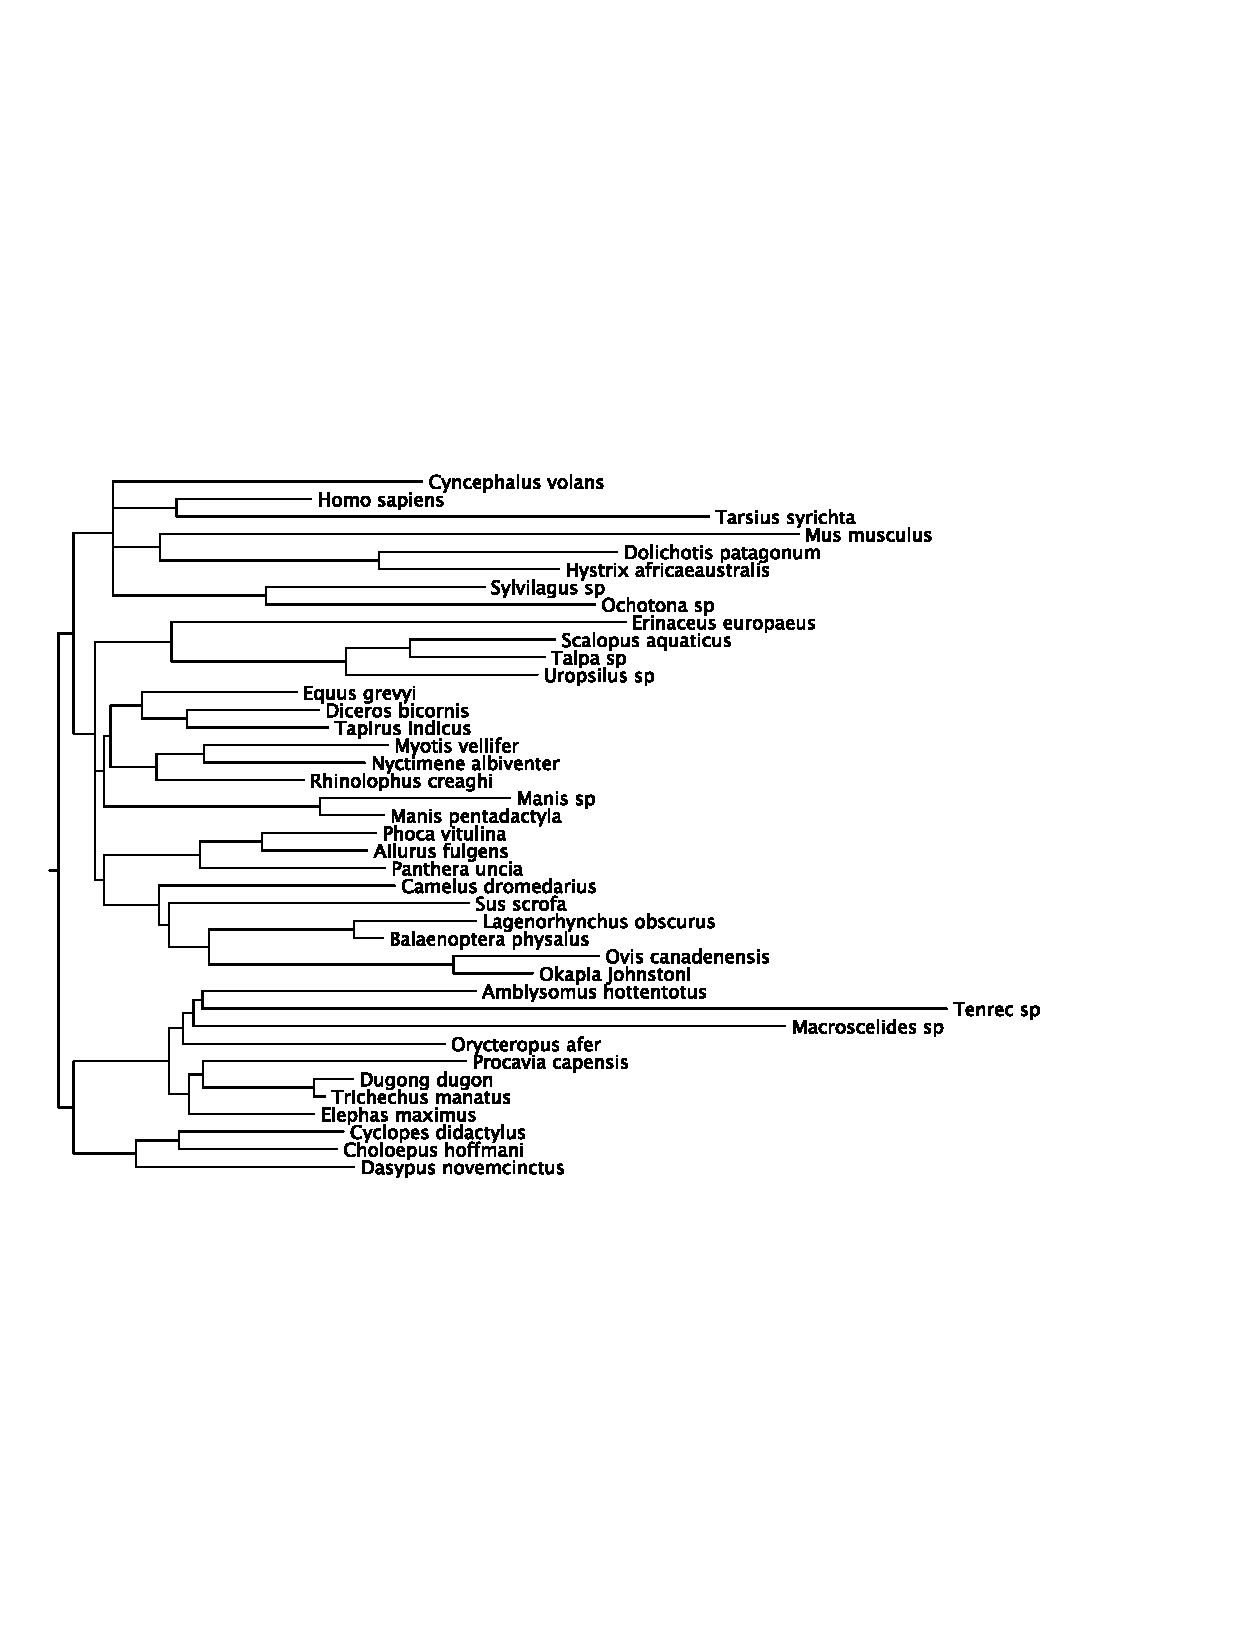
\includegraphics[width=28em]{waddellTree}
}
\headerbox{Results for the Symmetric Case}{name=results2,span=2,column=1,below=results}{
Although still in the process of completing the specialization for the symmetric case, we are now able to sketch out a rough computational complexity for it.  We have found here that the distinct subsets do not need considering.  Rather, it is only necessary to focus on the actual number of observed states, and to count the size of the subsets.  So, we need only to store information about each bin of probabilities, as opposed to having to store each of the state sets.  This unveils the potential for drastic improvement and simplification in the algorithm.


There are (n-1) internal nodes in a tree, which increases by a factor of one with each additional leaf on the tree.  (This is scaled linearly).  We must sweep over all the possible parsimony lengths under that, which are equal to [1-(the number of leaves at that point)].  Therefore, at each child we will need to calculate for 0 and 1, whereas at the ancestor we will need to calculate for 0, 1, 2 and 3.  But as the tree becomes very large, the number of calculations / the number of length bins will be approximately of the order n.  
}
\headerbox{Future Work}{name=results3,column=3,row=0}{
\begin{itemize}
\item We will continue to work on polishing the algorithm for the symmetric model.  This will include counting the size of the subsets, 
\item We plan to include our approaches in the GARLI \citep{GARLI} software package to be used in inferring evolutionary trees.  
\item We will also apply the model adequacy approach of Waddell {\em et al.~}\citep{WaddellOP2009}, as well as Felsenstein's \citep{Felsenstein1981} pruning algorithm to larger data sets, in order to have a better idea of certain evolutionary behaviors.
\end{itemize}
}

\headerbox{Acknowledgements}{name=acknowledgements,column=3,below=results3}{
\smaller						% Make the whole text smaller
\vspace{-0.4em}			% Save some space at the beginning
NSF

IMSD
} 

\headerbox{References}{name=references,column=3,below=acknowledgements}{
\smaller													% Make the whole text smaller
\vspace{-0.4em} 										% Save some space at the beginning
\bibliographystyle{plain}							% Use plain style
\renewcommand{\section}[2]{\vskip 0.05em}		% Omit "References" title
\bibliography{../pattern_class}
}



\end{poster}
\end{document}
